\documentclass{article}
%导言区插入下面三行
\usepackage{graphicx} %插入图片的宏包
\usepackage{float} %设置图片浮动位置的宏包
\usepackage{subfigure} %插入多图时用子图显示的宏包

\begin{document}

\begin{figure}[H] %H为当前位置,!htb为忽略美学标准,htbp为浮动图形
    \centering %图片居中
    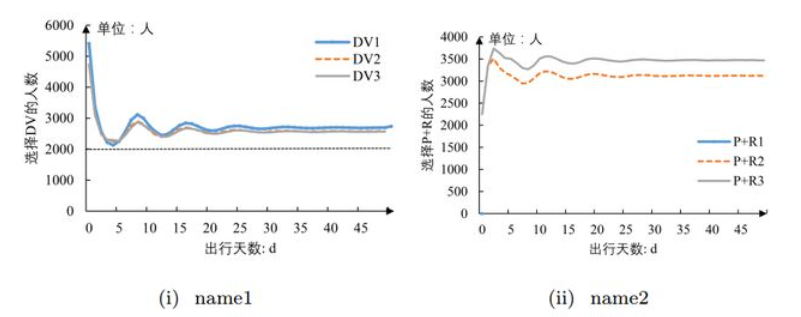
\includegraphics[width=0.7\textwidth]{DV_demand} %插入图片,[]中设置图片大小,{}中是图片文件名
    \caption{Main name 2} %最终文档中希望显示的图片标题
    \label{Fig.main2} %用于文内引用的标签
\end{figure}

\end{document}